% Введение.
\newpage
\section*{Введение}                      % выключить номер введения
\addcontentsline{toc}{section}{Введение} % но добавить его в оглавление

% --- Абзац приоритеты.

Высокопроизводительные вычисления \cite{GOST57700HPC} являются важным инструментом, применяемым в научных исследованиях и промышленных разработках для изучения сложных ресурсоемких процессов.

% а) переход к передовым технологиям проектирования и создания высокотехнологичной продукции.
Высокопроизводительные вычисления являются основой для развития передовых технологий проектирования и создания высокотехнологичной продукции.
В частности они применяются в авиационной и космической промышленности \cite{Kornev2021SuperAvio}, автомобилестроении \cite{Wang2020SuperAuto}, проектировании морского и железнодорожного транспорта, турбин и других высокотехнологичных изделий.
Важную роль высокопроизводительные вычислительные системы играют при проектировании образцов вооружения, в частности военной техники и боеприпасов \cite{Ageeva2023SuperMilitary}.
Также высокопроизводительные вычисления незаменимы при разработке новых материалов, для изучения свойств которых требуется проводить точное атомистическое моделивование структур, состоящих из миллиардов отдельных атомов \cite{Wang2025SuperMolDyn}.

% б) переход к экологически чистой и ресурсосберегающей энергетике, повышение эффективности добычи и глубокой переработки углеводородного сырья, формирование новых источников энергии, способов ее передачи и хранения.
В энергетической сфере высокопроизводительные вычисления применяются для моделирования объектов генерации электроэнергии, включая атомные станции \cite{Cancemi2025SuperNuc} в совокупности с процессами внутри ядерных реакторов, ветряные и приливные генераторы \cite{Quint2025SuperWind}.
Детальное моделирование месторождений углеводородного сырья позволяет повысить эффективность добычи \cite{Usmanov2024SuperPlast}, а создание цифровых моделей месторождений и систем транспортировки \cite{Didenko2023SuperOil} приводит к снижению потерь и обеспечивает прозрачность полного жизненного цикла, начиная с добычи сырья и заканчивая реализацией конечного продукта.

% в) переход к персонализированной, предиктивной и профилактической медицине, высокотехнологичному здравоохранению и технологиям здоровьесбережения, в том числе за счет рационального применения лекарственных препаратов.
Использование больших вычислительных систем позволило извлекать качественно новые данные из точного моделирования крупных органических молекул и их ансамблей \cite{Teplukhin2009SuperBigMolec}.
Во время борьбы с пандемией COVID-19\label{abbr:covid-1} высокопроизводительные вычисления играли передовую роль в изучении вируса и разработке вакцины \cite{Colonnelli2021SuperCovid}.
Обработка с помощью искусственного интеллекта больших массивов медицинских данных, включая истории болезней, медицинские анализы и снимки \cite{Ri2024SuperXRay}, в совокупности с геномными исследованиями в настоящее время знаменует переход к персонализированной медицине \cite{Kishore2024SuperPrecMed}.

% г) переход к высокопродуктивному и экологически чистому агро- и аквахозяйству, разработку и внедрение систем рационального применения средств химической и биологической защиты сельскохозяйственных растений и животных, хранение и эффективную переработку сельскохозяйственной продукции.
Компьютерное моделирование активно используется в растениеводстве и животноводстве для повышения эффективности выработки продовольствия.
Сюда входит целый спектр применений, начиная от селекции растений и животных \cite{Ahmetshina2020SuperSelection}, мониторинга их здоровья \cite{Mourant2018SuperEpi}, разработки удобрений и кормов \cite{Irfan2016SuperFert} и заканчивая планированием графиков разведения животных и выращивания сельскохозяйственных культур \cite{Zhang2021SuperFertPlan}.

% д) противодействие техногенным, биогенным, социокультурным угрозам, терроризму и экстремистской идеологии, деструктивному иностранному информационно-психологическому воздействию, а также киберугрозам и иным источникам опасности для общества, экономики и государства, укрепление обороноспособности и национальной безопасности страны в условиях роста гибридных угроз.
В связи со быстрым распространением цифровизации во всех областях современной жизни и ростом объема цифровых данных особую важность обретает задача обеспечения кибербеопасности и сохранности данных.
Злонамеренные действия в киберсреде могут привести к серьезным последствиям, включая финансовые потери, техногенные и экологические катастрофы.
Высокопроизводительные вычисления используются для исследования и создания новых инструментов информационной безопасности, в том числе с помощью технологий искусственного интеллекта и систем распределенного реестра \cite{Terziyska2024SuperCyber}.

% е) повышение уровня связанности территории Российской Федерации путем создания интеллектуальных транспортных, энергетических и телекоммуникационных систем, а также занятия и удержания лидерских позиций в создании международных транспортно-логистических систем, освоении и использовании космического и воздушного пространства, Мирового океана, Арктики и Антарктики.
Ввиду обширности территории России и неравномерности ее заселения и инфраструктурного обеспечения, необходимо создание интеллектуальных транспортных и телекоммуникационых систем для повышения уровня связности территории.
Высокопроизводительные вычисления применяются для проектирования и развития систем железнодорожного и авиасообщения \cite{Juntana2022SuperFlight}, обеспечения логистики морских перевозок \cite{Yan2024SuperSea}, а также для создания глобальных компьютерных сетей \cite{Abramov2025SuperNets}.

% ж) возможность эффективного ответа российского общества на большие вызовы с учетом возрастающей актуальности синтетических научных дисциплин, созданных на стыке психологии, социологии, политологии, истории и научных исследований, связанных с этическими аспектами научно-технологического развития, изменениями социальных, политических и экономических отношений.
%Развитие цифровизации во всем мире затрагивает не только технические стороны жизни человека, но и социально-психологические аспекты.
%В настоящее время можно констатировать, что социально-психологический профиль человека практически полностью определяется по его цифровому следу.
%Это с одной стороны открывает возможности по моделированию социальных и политических процессов \cite{} на основе цифровых данных.
%С другой стороны, доступность цифровых данных создает уязвимости как отдельного человека, так и целых групп населения, поэтому такие угрозы также нужно %анализировать и парировать \cite{}.

% з) объективную оценку выбросов и поглощения климатически активных веществ, снижение их негативного воздействия на окружающую среду и климат, повышение возможности качественной адаптации экосистем, населения и отраслей экономики к климатическим изменениям.
Техногенное влияние человека на окружающую среду постоянно возрастает, и высокопроизводительные вычисления применяются для решения задач экологии.
С помощью компьютерного моделирования и глобальных моделей проводятся исследования климата \cite{Kulkarni2024SuperClimate}, мирового океана \cite{Wei2024SuperOcean}, экосистем \cite{Rahman2024SuperSpecies} и оцениваются выбросы в окружающую среду и их последствия \cite{Ostromsky2024SuperAir}.

% и) переход к развитию природоподобных технологий, воспроизводящих системы и процессы живой природы в виде технических систем и технологических процессов, интегрированных в природную среду и естественный природный ресурсооборот.
%В последнее время особый акцент в технологическом развитии делается на природоподобные технологии, основанные на воспроизведении систем и процессов живой природы.
%Как правило, эти системы и процессы состоят из большого количества взаимодействующих элементов, которые требуют точного моделирования, что возможно только с использованием суперкомпьютеров.
%К природоподобным направлениям, связанным с высокопроизводительными вычислениями, можно отнести разработку нейроморфных процессоров~\cite{Rhodes2019SuperNuero}, технологии синтеза и воспроизведения тканей и органов человека \cite{Wang2012SuperTissues}, топологическую оптимизацию в проектировании изделий и строительстве \cite{Fedchikov2024SuperBim} и другие направления.

% Суррогатные вычисления.
%Широкое применение суперкомпьютерного моделирования в проектировании сложных технических систем связано с задачей выбора оптимальной конфигурации при большом количестве входных параметров.
%По мере усложнения проектируемых систем и роста количества параметров возникла проблема дефицита вычислительных ресурсов, что привело к появлению концепции суррогатного моделирования \cite{Jiang2020Surrogate,Barcenas2023Surrogate,Catalani2024Surrogate}, то есть использования упрощенных суррогатных моделей, обученных на результатах суперкомпьютерного моделирования на ограниченных наборах данных.
%Но даже использование суррогатного моделирования может лишь частично снизить потребность в вычислительных ресурсах и не умаляет актуальность проблемы эффективного их использования.

%Приведенный выше, но далеко не полный перечень сфер применения высокопроизводительных вычислений отражает основные приоритеты научно-технологического развития Российской Федерации.
%Развитие суперкомпьютерных технологий необходимо для обеспечения места России среди мировых технологических лидеров, поэтому вопросы создания и эффективного использования высокопроизводительных вычислительных систем являются крайне актуальными, особенно в условиях настоящего дефицита высокопроизводительных ресурсов в Российской Федерации \cite{Voevodin2021SuperRussia}.

Таким образом, сферы применения высокопроизводительных вычислений соответствуют приоритетам научно-технологического развития Российской Федерации и в частности переходу к передовым технологиям проектирования и создания высокотехнологичной продукции на основе интеллектуальных производственных решений, роботизированных и высокопроизводительных вычислительных систем, новых материалов и химических соединений, результатов обработки больших объемов данных, технологий машинного обучения и искусственного интеллекта.
Развитие суперкомпьютерных технологий необходимо для обеспечения России места среди мировых технологических лидеров, вопросы создания и эффективного использования высокопроизводительных вычислительных систем актуальны и вынесены на государственный уровень.

% --- Абзац расчеты в пространстве и на поверхности.

Компьютерное моделирование физических процессов в трехмерном пространстве относится к наиболее ресурсоемким научно-техническим задачам, связанным с высокопроизводительными вычислениями.
В числе таких задач можно назвать моделирование процессов газовой динамики \cite{Lobanova2023GeneralGas}, электромагнетизма \cite{Taboada2013GeneralElectro}, термодинамики \cite{Liu2020GeneralThermo} и многих других.
При этом вычисления проводятся, как правило, с использованием расчетных сеток, которые могут описывать как область трехмерного пространства (объемные расчетные сетки \cite{Kudryavzeva2014GeneralVolumeMesh}), так и некоторую расположенную в трехмерном пространстве поверхность (поверхностные расчетные сетки \cite{Zheleznyakova2016GeneralSurfMesh}).
Особую сложность при проведении компьютерного моделирования представляет организация вычислений при работе с динамическими расчетными сетками -- адаптивными сетками \cite{Li2014Film} и сетками с изменяющейся геометрией.
Одним из практически важных применений динамических расчетных сеток в компьютерном моделировании является задача моделирования обледенения поверхности \cite{Koshelev2020Ice}.
Вычисления по моделированию обледенения проводятся на поверхностных неструктурированных расчетных сетках с изменяющейся геометрией, описывающих поверхность в трехмерном пространстве, а также на объемных расчетных сетках, описывающих область пространства вокруг этой поверхности.

\paragraph{Актуальность темы} \

% --- Абзац безопасность полетов.

Задача моделирования обледенения летательных аппаратов является критически важной для обеспечения безопасности полетов \cite{Raj2020IntroIce}.
Известны случаи, когда обледенение несущих частей и силовых установок летательных аппаратов приводили к авиакатастрофам с большим количеством человеческих жертв,
%\footnote[1]{Катастрофа Ан-148 в Подмосковье в 2018 г., катастрофа DC-8 в Канаде в 1985 г., катастрофа Ту-134 под Минском в 1985 г., катастрофа MD-83 в Мали в 2014 г., катастрофа Ан-24 в Бугульме в 1991 г.}
что свидетельствует о важности этой задачи и востребованности результатов ее решения.
Требования и рекомендации к процессам проектирования, разработки и сертификации авиационных систем с учетом эксплуатации в режимах обледенения зафиксированы во многих нормативных документах.
%\footnote[2]{14 CFR -- Part 25 (Appendix C, O), Part 29 (Appendix C), Part 33 (Appendix D); FAA AC 25-28; ARP 4754; ARP 4761; Р 4761; ISO 11076:2020; Doc 9640; FAA Report ADS-4; FAA Report RD-77-76; НЛГ БАС-СТ.}.

% --- Абзац комплексность.

Задача обледенения поверхности является комплексной.
Для получения адекватной картины обледенения необходимо учитывать множество связанных между собой процессов, включая обтекание тела, выпадение на поверхность влаги и ледяных кристаллов из окружающего потока \cite{Cui2023Impingement}, взаимодействие выпадающего вещества с поверхностью \cite{Cui2021Impingement}, течение жидкости по поверхности в виде тонкой пленки или отдельных нитей \cite{Alexeenko2013Ice}, теплопроводность на поверхности, а также через слой жидкости и льда \cite{Xin2013Ice} и другие процессы.
В процессе образования слоя льда меняется геометрия рассматриваемой поверхности, так как форма образовавшихся ледяных наростов влияет на все связанные процессы, что приводит к необходимости перестроения расчетных сеток.

% --- Абзац другие пакеты.

В пользу актуальности и востребованности исследований и разработок в области моделирования обледенения свидетельствует большое количество существующих и разрабатываемых программных пакетов для решения этой проблемы.
К таким решениям относятся пакет инженерного проектирования ANSYS (включающий в себя модули FENSAP-ICE, DROP3D, ICE3D) \cite{Martini2022IntroIce}, модуль iceFoam \cite{Koshelev2020Ice} как часть открытого программного обеспечения OpenFOAM\label{abbr:foam-1}, решение для моделирования обледенения в составе пакета инженерного анализа ЛОГОС \cite{Galanov2021IntroIce,Galanov2021IntoIceLOGOS}, модуль IceVision \cite{Sorokin2020Ice} в составе пакета FlowVision, а также ряд других пакетов решений, таких как LEWICE \cite{Shannon2019IntroIce}, AIPAC \cite{Domingos2015IceHeat}, ONERA \cite{Villedieu2014IntroIce}, TRAJICE \cite{Son2010IntroIce}.

% --- Абзац макроитерации.

Моделирование обледенения выполняется, как правило, на поверхностных расчетных сетках и состоит из отдельных макроитераций, каждая из которых проходит в два этапа.
На первом этапе выполняется расчет интенсивности нарастания льда в рамках отдельных ячеек расчетной сетки.
Для вычисления интенсивности ледообразования в ячейках расчетной сетки существует множество моделей обледенения \cite{Bartkus2018IntroIce,Zhang2017IntroIce,Pena2016IntroIce}, в которых учитываются различные состояния льда, течение жидкой пленки по поверхности, тепловые потоки, выпадение на поверхность влаги, ледяных кристаллов и переохлажденных капель \cite{Wang2023IntroIce,Liu2022IntroIce}, различные механики плавления и срыва ледяных наростов \cite{Ruan2023IntroIce} и многие другие факторы.
Результатом первого этапа макроитерации является информация о количестве льда, накопленного в каждой ячейке расчетной сетки.
На втором этапе макроитерации выполняется перестроение поверхности обледеневающего тела.
При этом перестроение должно выполняться таким образом, чтобы изменение объема рассматриваемого тела соответствовало вычисленному на первом этапе макроитерации объему накопленного в ячейках льда.
После перестроения поверхностной расчетной сетки необходимо произвести пересчет поля скоростей вокруг нее, так как изменение геометрии поверхности существенным образом влияет на картину обтекания.
После пересчета поля скоростей моделирование обледенения может быть продолжено.

%\begin{figure}[ht]
%\centering
%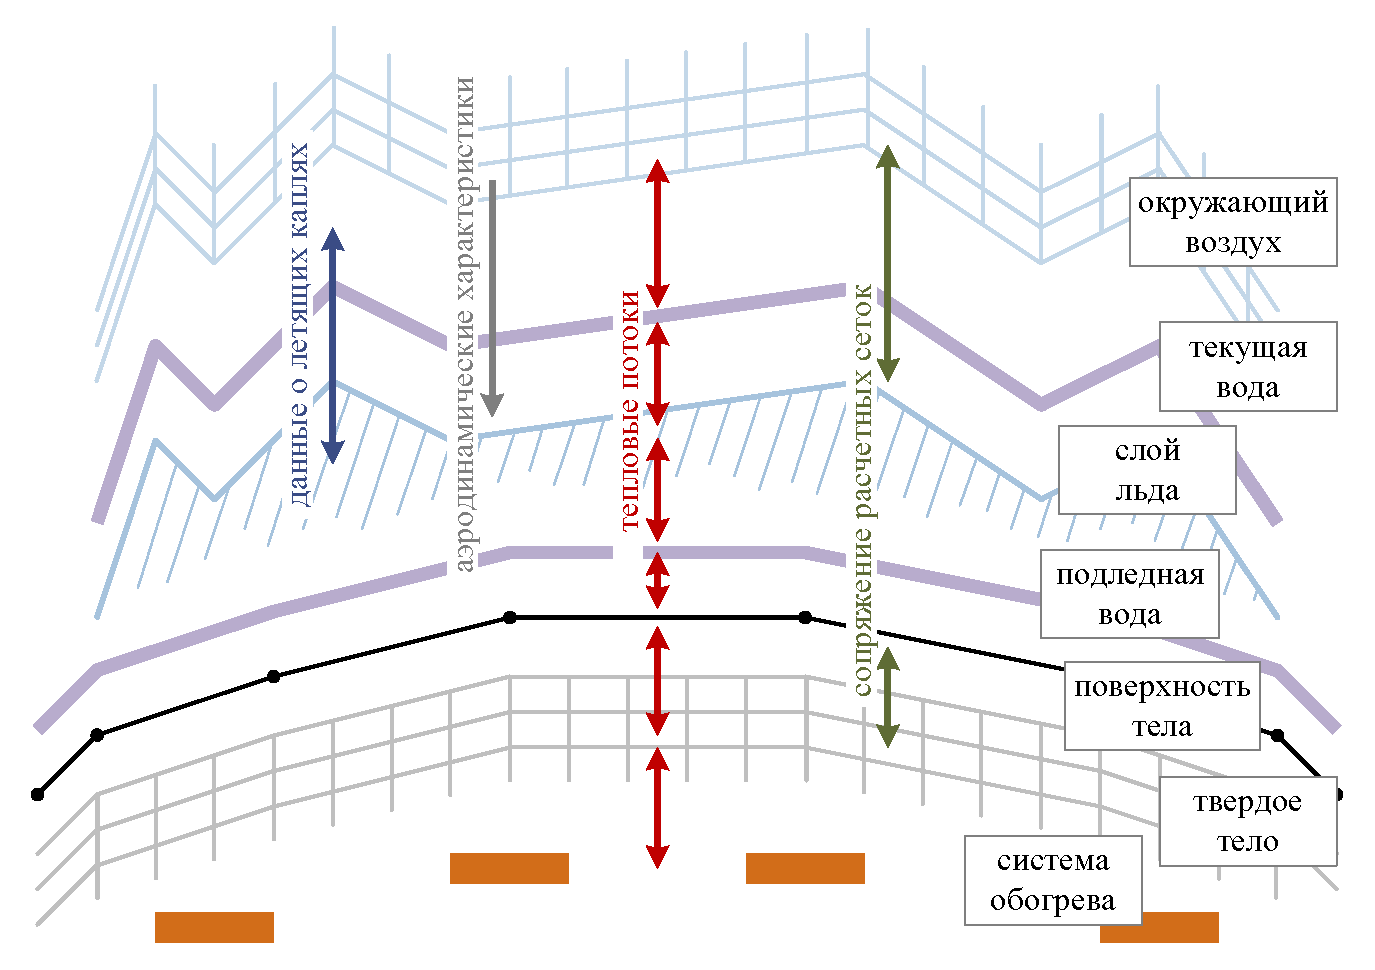
\includegraphics[width=1.0\textwidth]{pics/text_0/multi-scheme.pdf}
%\singlespacing
%\captionstyle{center}\caption{Многослойная модель ледообразования.}
%\label{fig:text_0_multi_scheme}
%\end{figure}

%Во время расчета первого этапа каждая ячейка поверхностной расчетной сетки представлена в виде сложной структуры, состоящей из следующих слоев, перечисленных снизу вверх: элементы системы обогрева внутри тела -- твердое тело -- слой находящейся подо льдом жидкости -- слой льда -- текущая по поверхности льда жидкость -- окружающее воздушное пространство (см. рис.~\ref{fig:text_0_multi_scheme}).
%В зависимости от используемой модели можно выделять и другие слои.
%Во время выполнения расчетов осуществляется обмен потоками вещества и тепла между отдельными слоями, а также между соседними ячейками.

% --- Абзац ресурсоемкость.

Компьютерное моделирование обледенения является крайне ресурсоемким и включает в себя не только выполнение вычислений на поверхностной расчетной сетке, но и постоянное перестроение поверхностной сетки, пересчет поля скоростей в окружающем пространстве и различных характеристик поверхности, таких как коэффициент улавливания влаги или коэффициент теплоотдачи.
Перестроение поверхностной расчетной сетки, адекватно описывающей геометрию образующихся ледяных наростов, должно отвечать критериям точности и стабильности.
Возникновение дефектов сетки, таких как острые пики и изломы, трещины и впадины, самопересечения сетки, может привести к нефизичным результатам или даже к аварийному завершению расчета и необходимости его перезапуска, что приводит к дополнительному потреблению вычислительных ресурсов. 
Для моделирования обледенения на значимом промежутке времени требуется использование существенных вычислительных ресурсов и применение методов повышения производительности вычислений на поверхностных и объемных расчетных сетках на всех уровнях распараллеливания: в модели с передачей сообщений, на общей памяти и на уровне отдельных инструкций.

Существенное влияние на развитие суперкомпьютерных технологий, включая создание методов и программного обеспечения для организации и повышения производительности вычислений, оказали работы известных советских и российских ученых Г.И.~Савина, А.А.~Самарского, А.И.~Аветисяна, Б.Н.~Четверушкина, И.А. Соколова, Б.М.~Шабанова, Вл.В.~Воеводина, М.В.~Якобовского, А.Н. Томилина, В.В.~Коренькова, Б.А.~Бабаяна, В.Ф. Тишкина. 

\paragraph{Цели и задачи работы} \

\input text_goal.tex

\input text_tasks.tex

\input text_methodology.tex

\input text_statements.tex

\input text_new.tex

\input text_spec_passport.tex

\input text_theoretical_practical.tex

\input text_true_results.tex

\input text_conferences.tex

%\input text_myown.tex

% Публикации.
\paragraph{Публикации} \

По теме диссертации автором опубликовано 35 печатных работ, из них 24 работы опубликованы в журналах, рекомендованных ВАК\label{abbr:vak-1} (в том числе 5 работ -- в журналах, входящих в список К1 перечня ВАК), 15 работ -- в журналах, входящих в индекс RSCI\label{abbr:rsci-1}, 7 работ -- в журналах, индексируемых в международных базах научных изданий Web of Science и Scopus.
По теме диссертации получено 7 свидетельств о государственной регистрации программ для ЭВМ\label{abbr:evm-1} \cite{CertGoryachev2023Crys,CertGoryachev2020Crys,CertRybakov2021PrepUnstruct,CertRybakov2020PrepStruct,CertRybakov2024Surf,CertRybakov2023Mon,CertRybakov2019AVX}.

\input text_struct.tex

\input text_brief_content.tex
